\subsection{Results}

\st{No results have been produced yet. More information will be provided following the launch campaign in a later version of the SED.}

\subsubsection{Expected Results}

It was expected that since atmospheric interference is a large contributor to the reduction of target light intensity and increased noise in the final images, flight images should have displayed increased clarity and finer detail, as well as an increased SNR as compared to images taken on the ground. 

\hl{
\subsection{Actual Results}
On October 25, 2019 at 04:21 UTC the BEXUS 28 balloon was launched. On its flight through the stratosphere, IRISC captured 75 near infra-red images in FITS format, in addition to the three dark frames taken in the hour before launch. In addition to commentary on the images acquired, there will also be discussion on the telemetry, specifically the mechanical behaviour of the telescope and its compliance with mission necessary specifications. Analysis was done using IDL Astronomy Users Library \texttt{astrolib}, modified for Gnu Data Language (GDL), for its FITS analysis capabilities. Other numerical analysis and graphs were done using GDL; images generated from FITS files using DS9.

\subsubsection{Dark Frames} 
All three dark frames presented with pixel values ranging from 1 to 4094, and mean pixel values of 44.254, 44.265, and 44.250, with corresponding standard deviations between 5.10 and 5.13. These values are within acceptable limits and are concurrent with an expected dark frame image. 

\begin{figure}[h]
\captionsetup[subfigure]{justification=centering}
\captionsetup{justification=centering}
    \centering
	\begin{subfigure}{0.49\textwidth}
		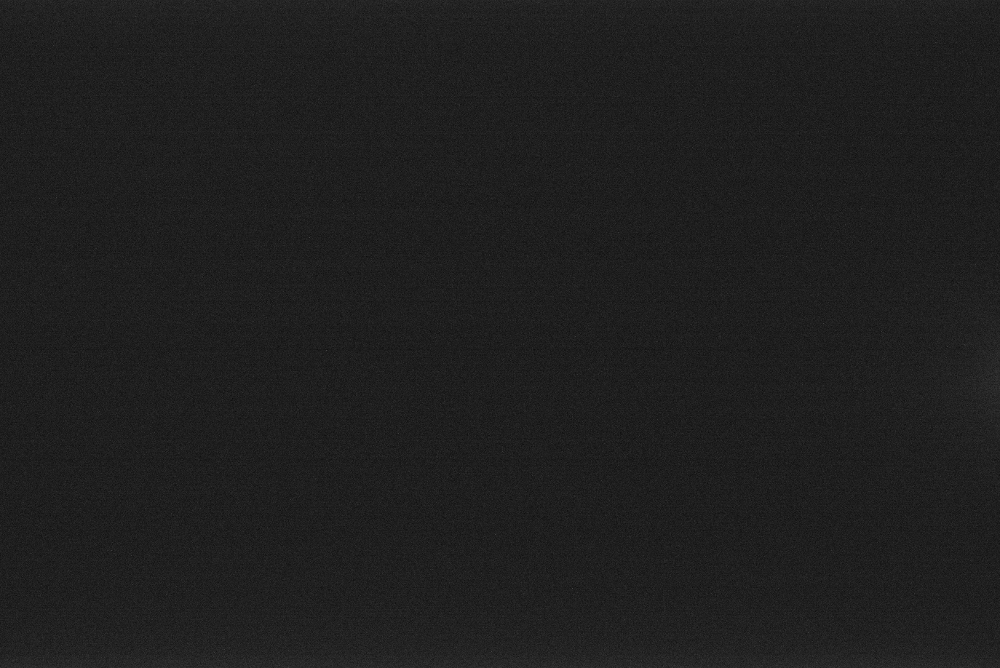
\includegraphics[width=1\linewidth]{appendix/img/campaign_results/d0.jpeg}
		\caption{First dark frame}
		\label{fig:sub:d0}
	\end{subfigure}
	\begin{subfigure}{0.49\textwidth}
		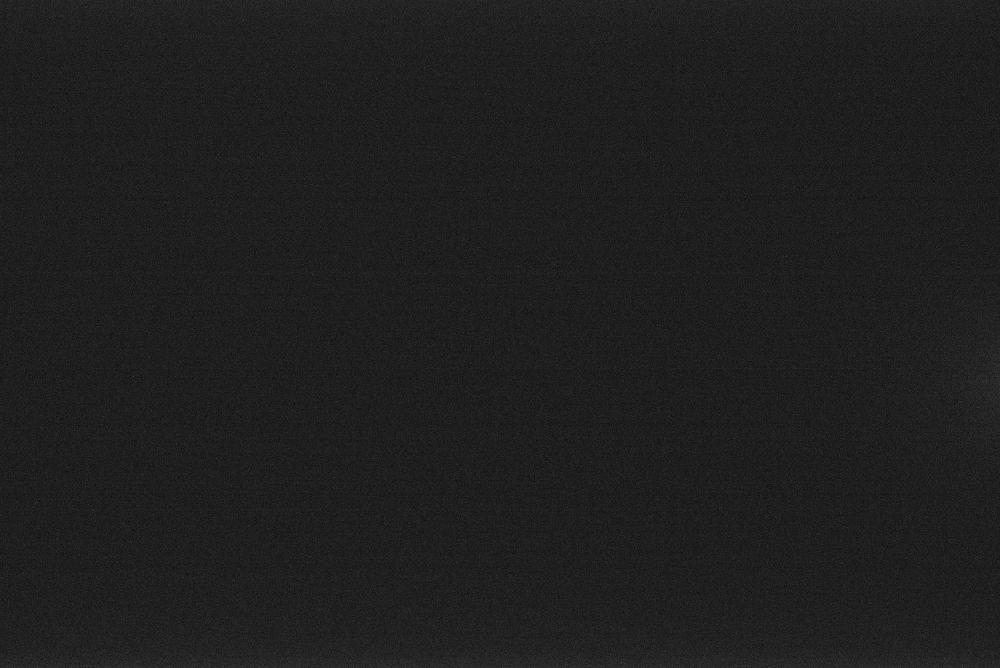
\includegraphics[width=1\linewidth]{appendix/img/campaign_results/d1.jpeg}
		\caption{Second dark frame}
		\label{fig:sub:d1}
	\end{subfigure}
	\begin{subfigure}{0.49\textwidth}
		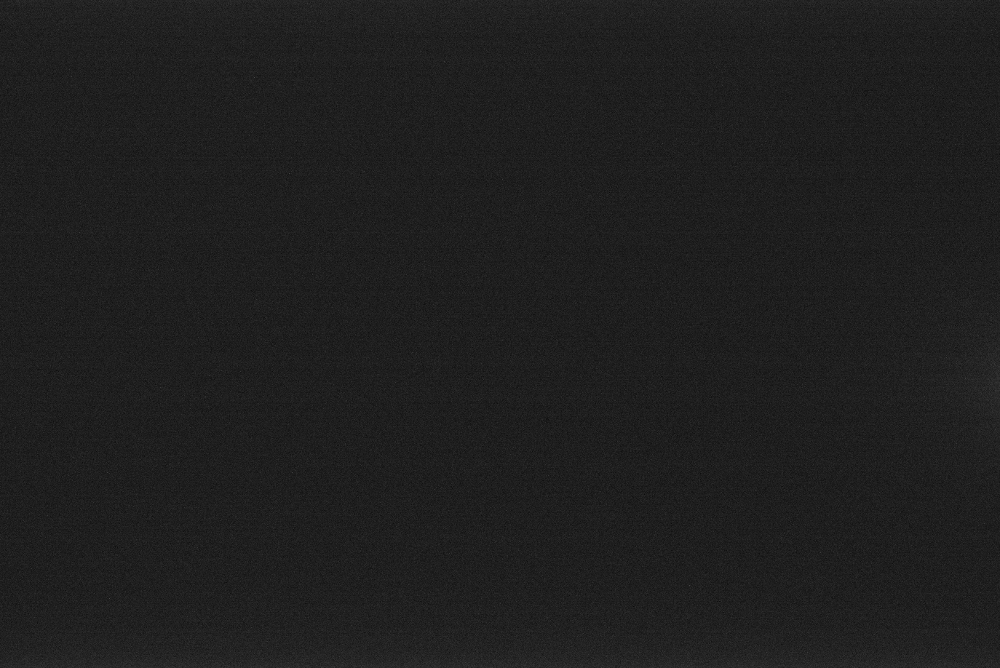
\includegraphics[width=1\linewidth]{appendix/img/campaign_results/d2.jpeg}
		\caption{Third dark frame}
		\label{fig:sub:d2}
	\end{subfigure}
	\caption{All three dark frames, as imaged by DS9 using a log scale centred at a pixel value of 45, for ease of visualisation}
\end{figure}

\subsubsection{Flight Images} 
Three images were corrupt upon delivery and could not be analysed. The 72 remaining non-corrupt images can be split into three exposure time categories: 15 with exposure time 30\,sec, 28 with exposure time 10\,sec, 29 with exposure time 1\,sec. All 72 images presented "blank"-- that is, all pixels in all images had a value of 4094, the highest pixel value. 

\newpage
\subsubsection{Flight Telemetry}

\subsubsection*{Encoder Logs:}
The encoder logs recorded the absolute angle of the telescope in the two axes relative to a certain offset point horizontal and normal to the gondola sidewall. A plot of the encoder log data for the duration of the flight reveals the motion of the telescope as pictured in figure \ref{fig:altaz}

\begin{figure}[htbp]
    \centering
    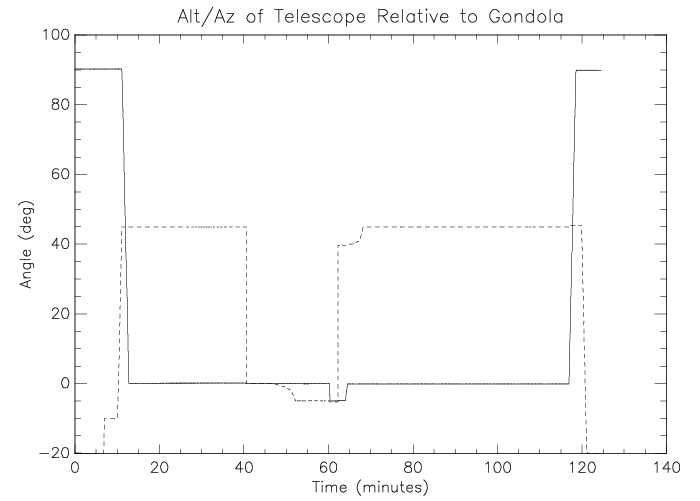
\includegraphics[width=0.9\textwidth]{appendix/img/campaign_results/altaz.jpg}
    \caption{Plot of azimuth angle (solid line) versus altitude/elevation angle (dotted line) of the telescope throughout the flight}
    \label{fig:altaz}
\end{figure}

\begin{figure}[htbp]
\captionsetup[subfigure]{justification=centering}
\captionsetup{justification=centering}
    \centering
	\begin{subfigure}{0.45\textwidth}
		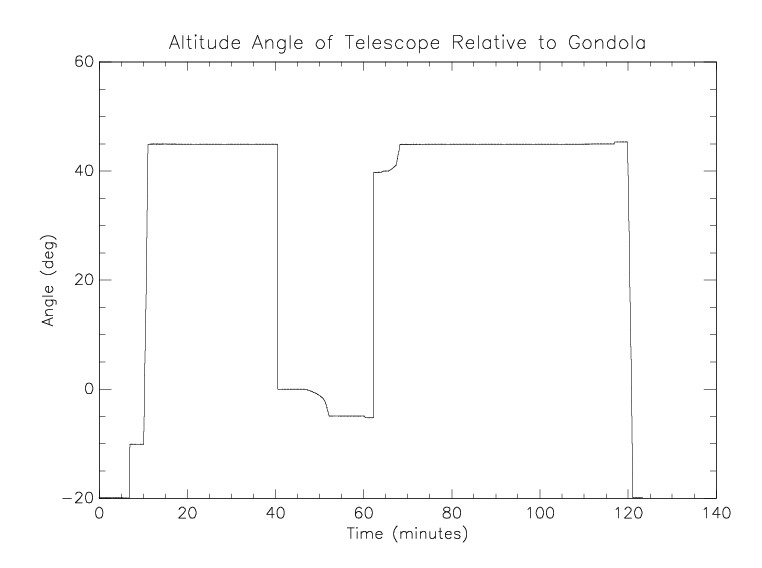
\includegraphics[width=1\linewidth]{appendix/img/campaign_results/altitude.jpg}
		\caption{Altitude angle alone}
		\label{fig:sub:alt}
	\end{subfigure}
	\begin{subfigure}{0.45\textwidth}
		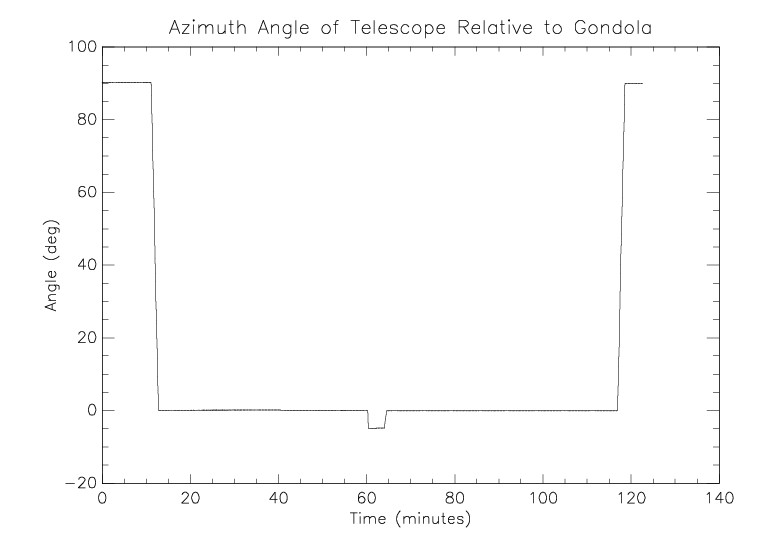
\includegraphics[width=1\linewidth]{appendix/img/campaign_results/azimuth.jpg}
		\caption{Azimuth angle alone}
		\label{fig:sub:az}
	\end{subfigure}
	\caption{Plots of each encoder axis on its own.}
\end{figure}

\subsubsection*{Temperature Logs:}
The temperature logs recorded the temperature across each of the NIR Camera, the Guiding Camera, and the CPU. Temperature recording began as soon as the system was powered on, before launch, as opposed to each of the encoder and gyroscope logs which began recording at given altitudes above the earth, after launch. However, figure \ref{fig:sub:gyrotemp} is temperature as recorded by the gyroscope logs rather than the temperature logs, and thus will have a different duration. 

\begin{figure}[htbp]
\captionsetup[subfigure]{justification=centering}
\captionsetup{justification=centering}
    \centering
    \begin{subfigure}{0.45\textwidth}
		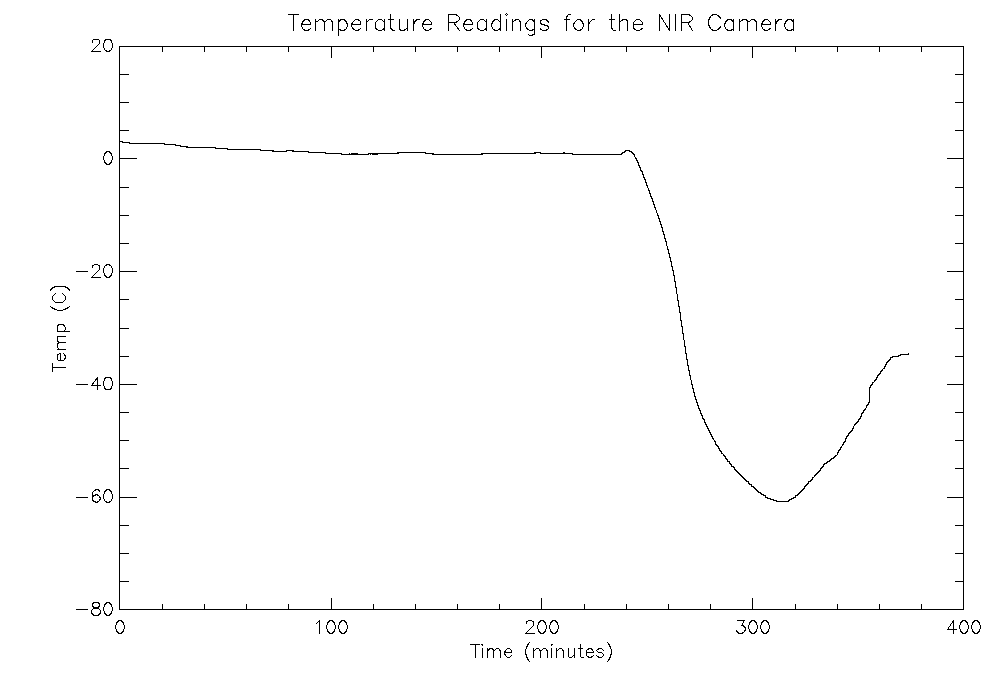
\includegraphics[width=1\linewidth]{appendix/img/campaign_results/tempnir.png}
		\caption{Temperature as recorded for the NIR Camera}
		\label{fig:sub:NIRtemp}
	\end{subfigure}
	\begin{subfigure}{0.45\textwidth}
		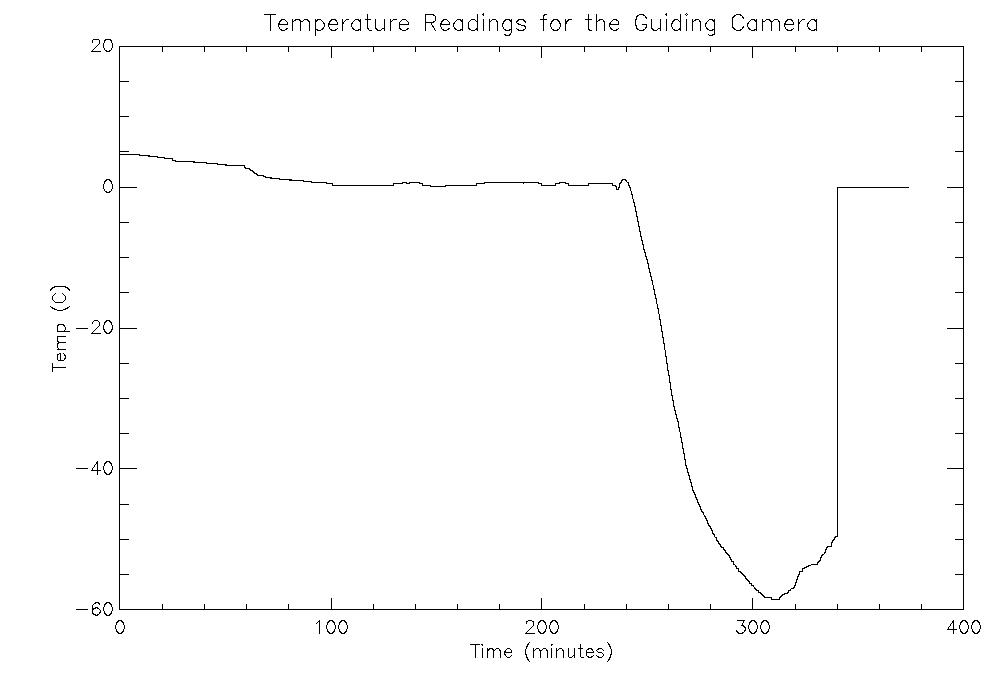
\includegraphics[width=1\linewidth]{appendix/img/campaign_results/tempgc.png}
		\caption{Temperature as recorded for the Guiding Camera}
		\label{fig:sub:GCTemp}
	\end{subfigure}
	\begin{subfigure}{0.45\textwidth}
		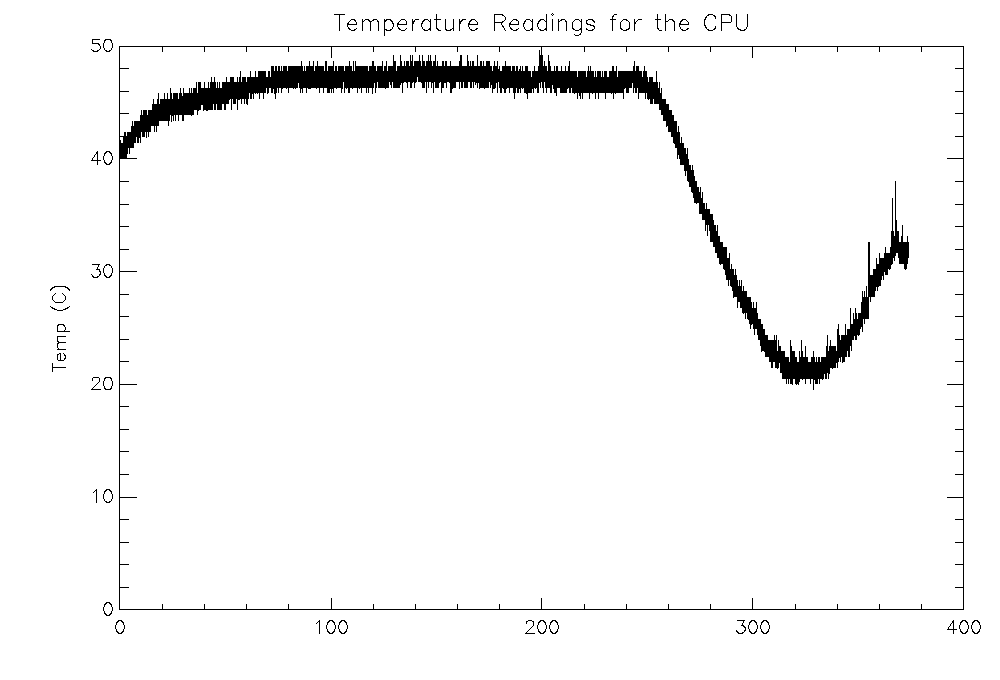
\includegraphics[width=1\linewidth]{appendix/img/campaign_results/tempcpu.png}
		\caption{Temperature as recorded for the CPU}
		\label{fig:sub:cputemp}
	\end{subfigure}
	\begin{subfigure}{0.45\textwidth}
		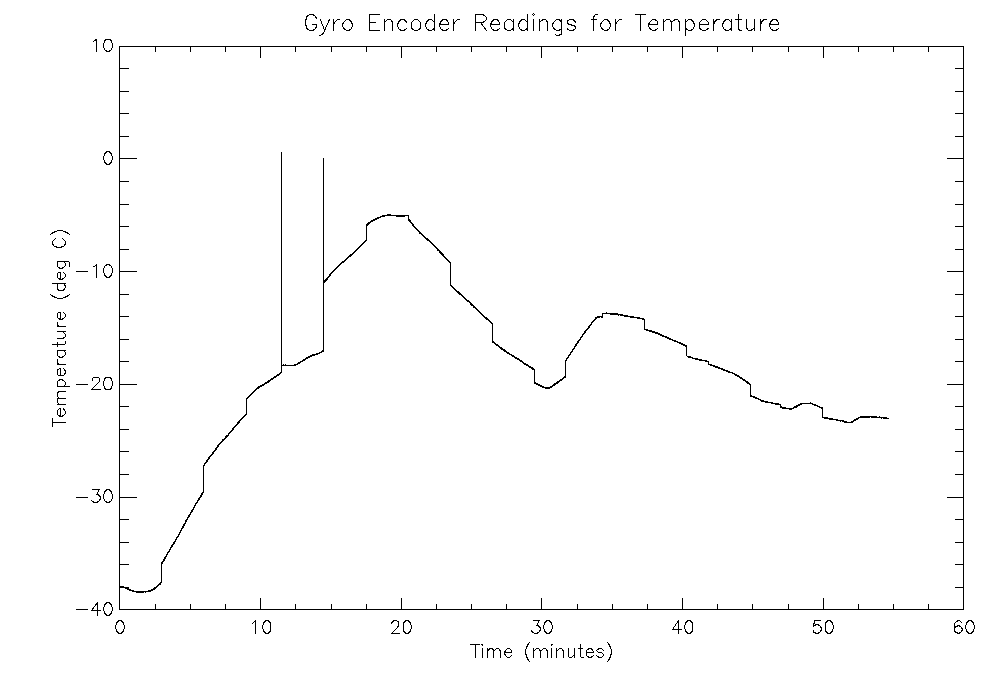
\includegraphics[width=1\linewidth]{appendix/img/campaign_results/gyrotemp.png}
		\caption{Temperature as recorded for the gyroscope}
		\label{fig:sub:gyrotemp}
	\end{subfigure}	
	\caption{Full results from temperature log for the duration of recording (note that time axis reflects different duration from that of encoder and gyroscope logs)}
	\label{fig:temp}
\end{figure}

\newpage
\subsubsection*{Gyro Logs:}
The gyroscope log recorded angular rate of each gyroscope axis: x(deg/s), y(deg/s), z(deg/s).

\begin{figure}[htbp]
\captionsetup[subfigure]{justification=centering}
\captionsetup{justification=centering}
    \centering
	\begin{subfigure}{0.45\textwidth}
		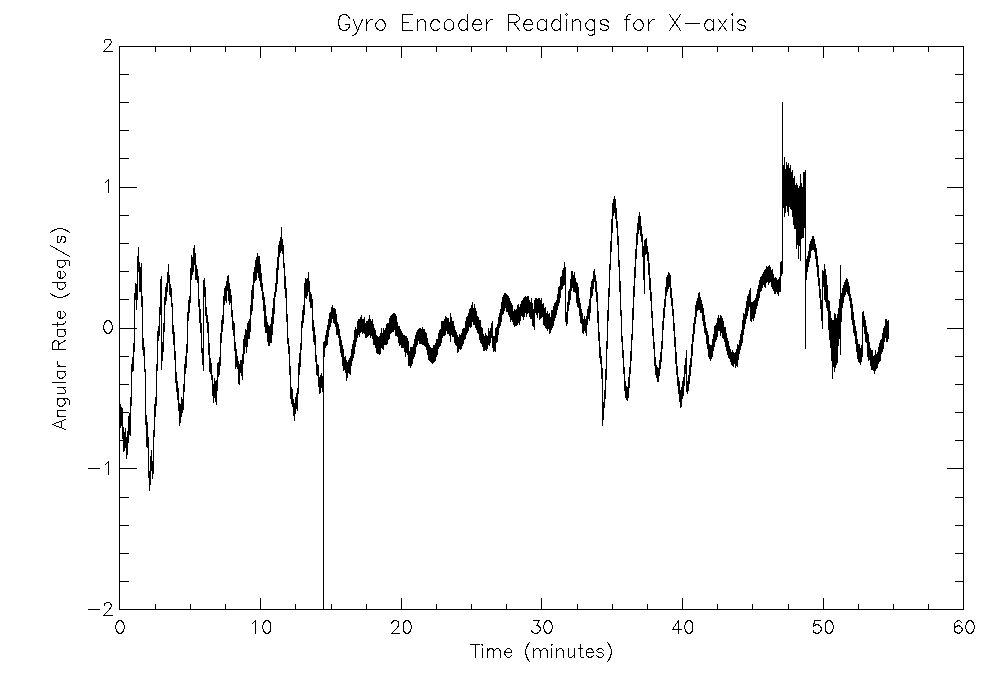
\includegraphics[width=1\linewidth]{appendix/img/campaign_results/gyrox.png}
		\caption{Angular rate of the gyro in the x-axis}
		\label{fig:sub:gyrox}
	\end{subfigure}
	\begin{subfigure}{0.45\textwidth}
		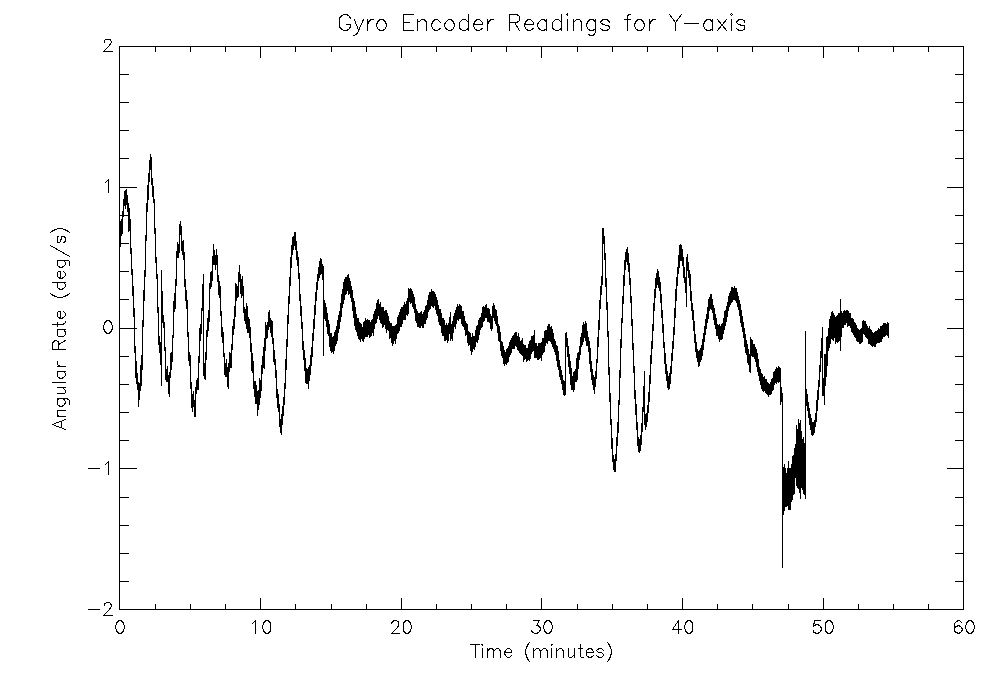
\includegraphics[width=1\linewidth]{appendix/img/campaign_results/gyroy.png}
		\caption{Angular rate of the gyro in the y-axis}
		\label{fig:sub:gyroy}
	\end{subfigure}
	\begin{subfigure}{0.45\textwidth}
		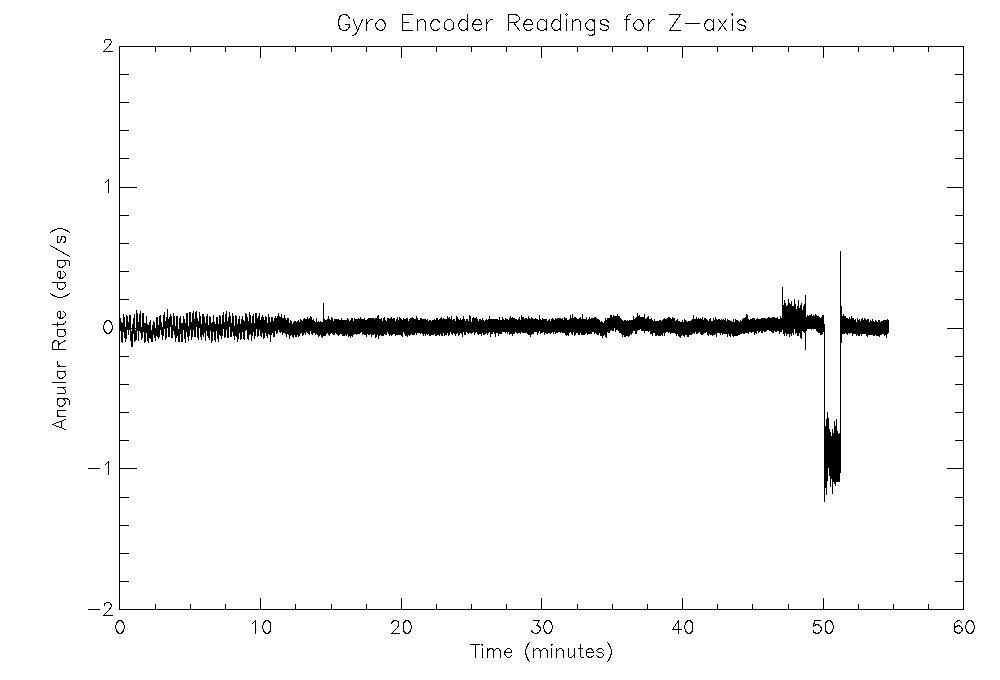
\includegraphics[width=1\linewidth]{appendix/img/campaign_results/gyroz.png}
		\caption{Angular rate of the gyro in the z-axis}
		\label{fig:sub:gyroz}
	\end{subfigure}
	\begin{subfigure}{0.45\textwidth}
		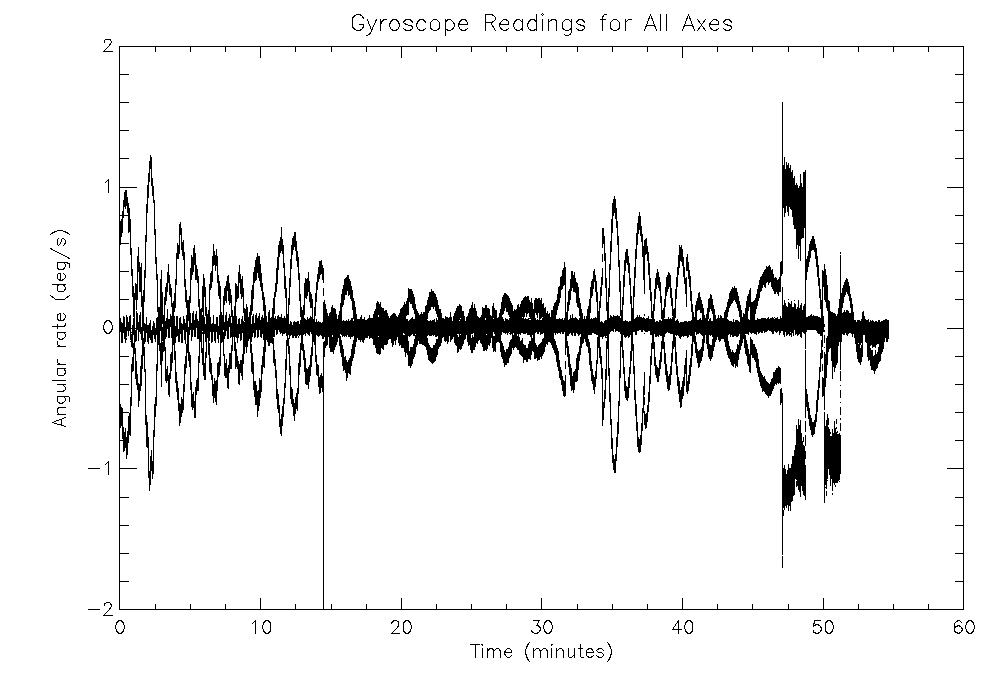
\includegraphics[width=1\linewidth]{appendix/img/campaign_results/gyroall.png}
		\caption{Overlaid image of each gyroscope axis}
		\label{fig:sub:gyroall}
	\end{subfigure}
	\caption{Full results from gyro log for the duration of recording (note that time axis reflects different duration from that of encoder and temperature logs)}
	\label{fig:gyro}
\end{figure}

\subsubsection*{PID Logs:}

The PID logs recorded the current position and target position as well as several other variables, but due to the nature of the flight, presented here is only the current position data. 

\begin{figure}[htbp]
\captionsetup[subfigure]{justification=centering}
\captionsetup{justification=centering}
    \centering
	\begin{subfigure}{0.45\textwidth}
		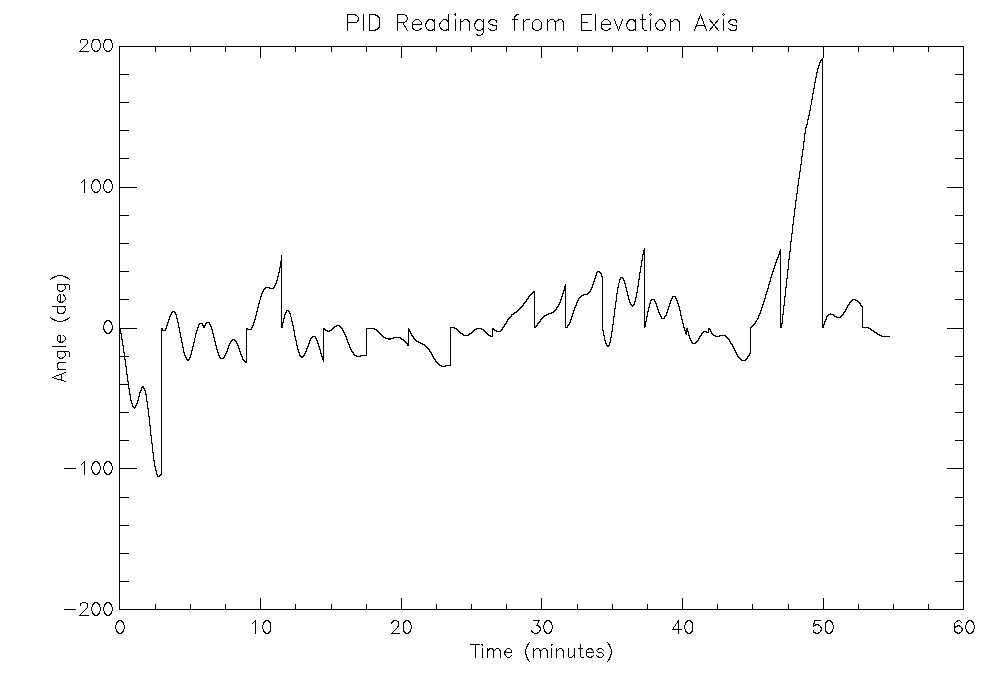
\includegraphics[width=1\linewidth]{appendix/img/campaign_results/pid_alt.png}
		\caption{PID log recordings for the altitude axis}
		\label{fig:sub:pidalt}
	\end{subfigure}
	\begin{subfigure}{0.45\textwidth}
		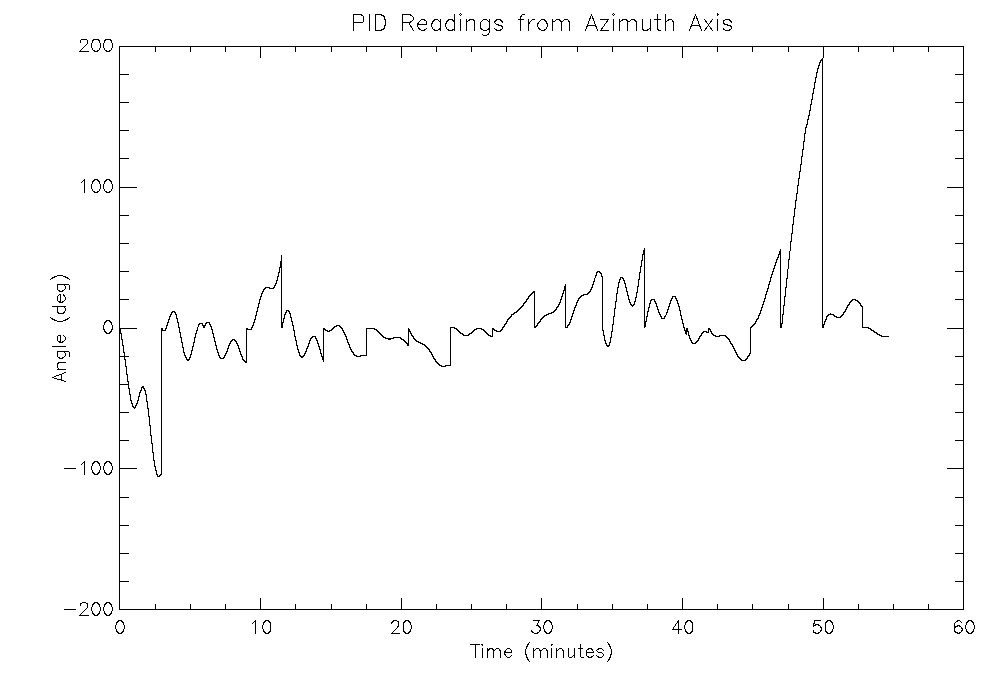
\includegraphics[width=1\linewidth]{appendix/img/campaign_results/pid_az.png}
		\caption{PID log recordings for the azimuth axis}
		\label{fig:sub:pidaz}
	\end{subfigure}
	\caption{Results from the PID log for the duration of recording (note that time axis reflects different duration from that of encoder and temperature logs)}
	\label{fig:PID}
\end{figure}

\subsubsection*{Star Tracker Performance}
As the guiding camera did not produce any images, the star tracker software never ran. Therefore, no analysis done on the performance of the star tracker.

\subsection{Analysis}

\subsubsection{Images}

Dark frame images showed low mean pixel values and low standard deviations, as expected for dark frame images. Unfortunately, all flight images presented with max pixel values for all pixels, meaning no scientific analysis can be done of any subjects within. These results might suggest over-exposure to the point of saturation, or perhaps a failure state of the electronic components.

Of interest here is that all in-flight images, even those with the lowest exposure of 1\,seconds, showed over-exposure. Given that the dark frames, all of which had exposure times of 10\,seconds, show a random spread of pixel values as opposed to ``hot spots" or the indications of an infrared source, one might expect that, with a suitable exposure time, in-flight images would present with the same random spread (or a more ordered image) and higher pixel values. However, even at a fraction of dark frame exposure time, over-exposure is present. This would suggest that, if over-exposure is the cause, then in-flight exposure times were too high, the telescope was pointed at a target of high infrared radiation, or both. 

Another possible explanation for the oddly consistent pixel values could be that this is indicative of partial failure of some components-- if external over-exposure was the cause, one might expect to see evidence of dead or fried pixels, which often report null or abnormal pixel values for a given image, even during over-exposure. Given that each and every pixel over ever image was the same, this does lend more credence to a failure state possibility. The most favoured possible cause of a failure state at present is sub-optimal environmental conditions, secondary to failed heating pads. The gyro temperature readings in figure \ref{fig:sub:gyrotemp} indicate that temperatures were at or below $-5^{\circ}$C for the entirety of the flight. The minimum operational temperature of the camera is $-5^{\circ}$C, so with failure of the heating equipment, the camera most likely would not have performed under these conditions. 

Post-flight testing of the camera revealed that the camera is still operational, giving further support to the idea that the transient nature of sub-optimal working temperatures caused a failure state and ``over-exposure" of the images during the flight. 

\newpage
\subsubsection{Logs}

\subsubsection*{Encoder logs}
The entire encoder log was split and truncated to isolate the two ``steady" configurations at approximately T:+25\,min to T:+40\,min (henceforth referred to as ``early flight"), and T:+87\,min to T:+106\,min (henceforth referred to as ``late flight"), to give approximately 35\,min total time in which to analyse and evaluate how steady the telescope was in-flight. These are visually presented in figure \ref{fig:fullsteady}.

\begin{figure}[h!]
\captionsetup[subfigure]{justification=centering}
\captionsetup{justification=centering}
    \centering
	\begin{subfigure}{0.45\textwidth}
		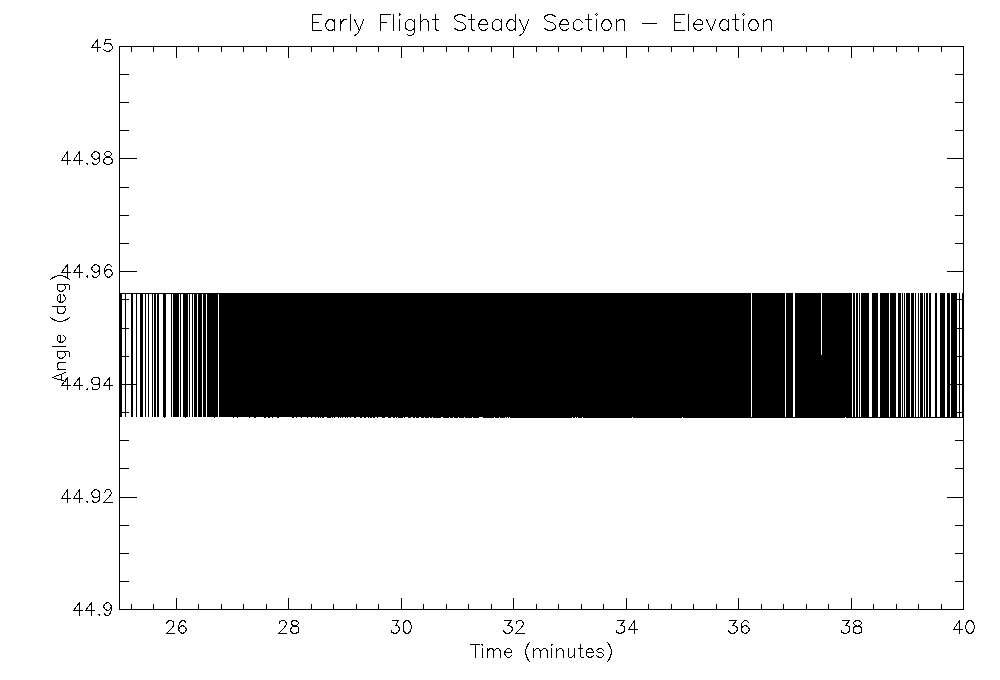
\includegraphics[width=1\linewidth]{appendix/img/campaign_results/earlyalt.png}
		\caption{Full length early flight angular deviation for elevation axis}
		\label{fig:sub:earlyalt}
	\end{subfigure}
	\begin{subfigure}{0.45\textwidth}
		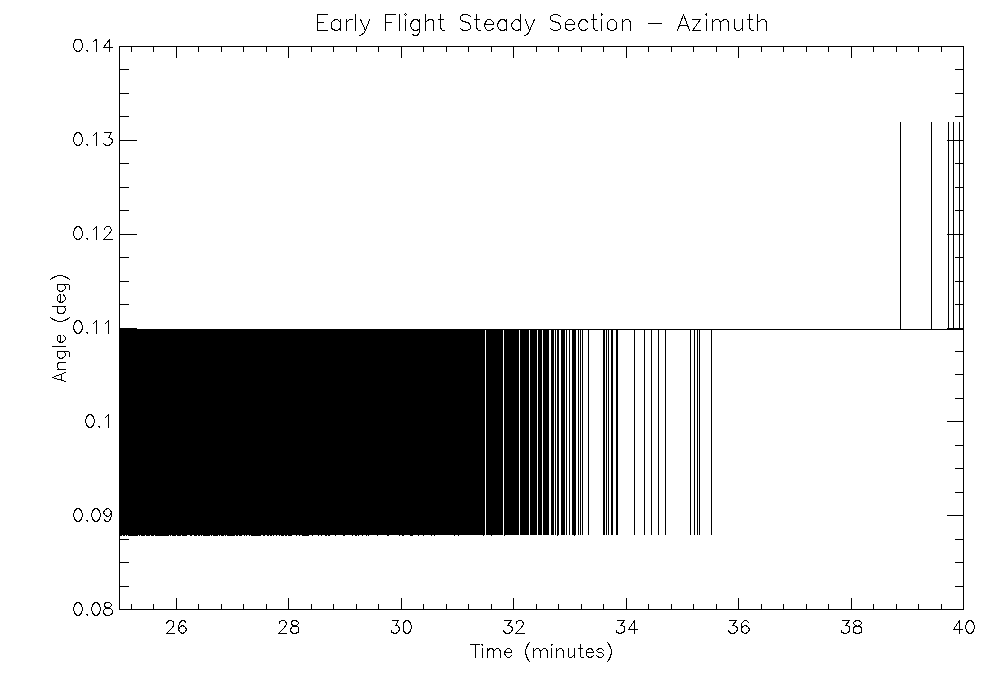
\includegraphics[width=1\linewidth]{appendix/img/campaign_results/earlyaz.png}
		\caption{Full length early flight angular deviation for azimuth axis}
		\label{fig:sub:earlyaz}
	\end{subfigure}
	\begin{subfigure}{0.45\textwidth}
		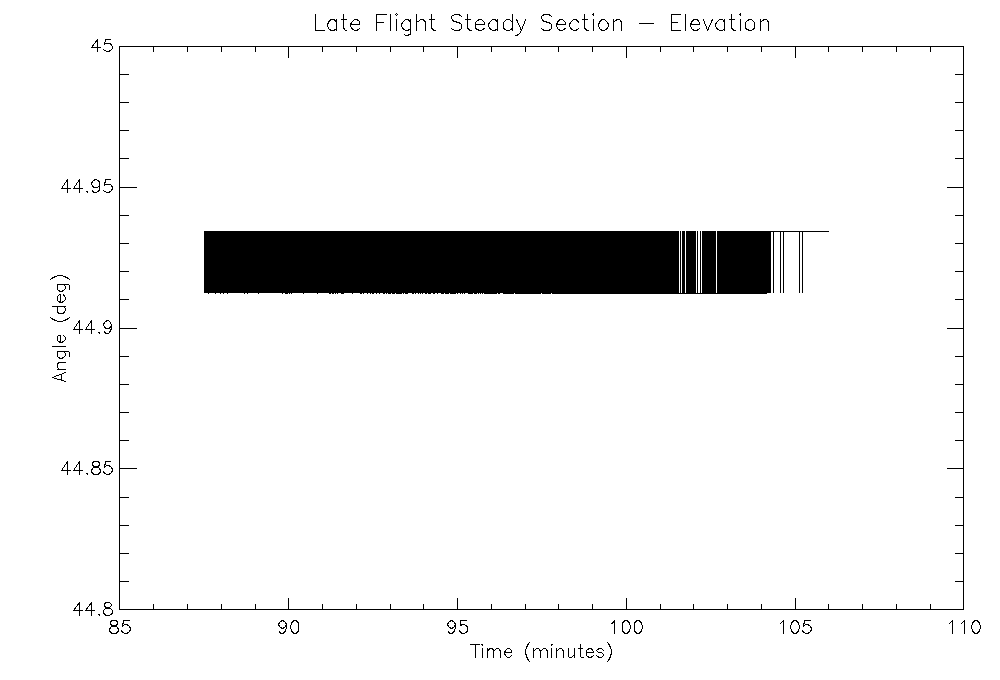
\includegraphics[width=1\linewidth]{appendix/img/campaign_results/latealt.png}
		\caption{Full length late flight angular deviation for elevation axis}
		\label{fig:sub:latealt}
	\end{subfigure}
	\begin{subfigure}{0.45\textwidth}
		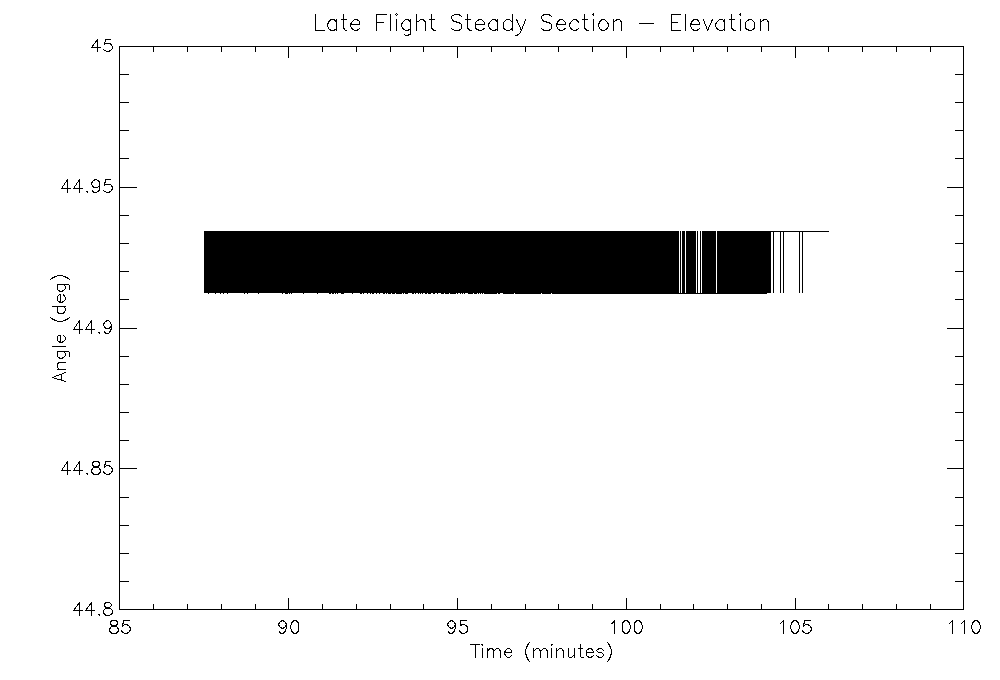
\includegraphics[width=1\linewidth]{appendix/img/campaign_results/latealt.png}
		\caption{Full length late flight angular deviation for azimuth axis}
		\label{fig:sub:lateaz}
	\end{subfigure}
	\caption{Full range of data for both steady portions of the flight}
	\label{fig:fullsteady}
\end{figure}

Whilst in this stationary state, the encoder logs presented with minute oscillations in position for the duration of the flight. Figures \ref{fig:earlyflight} and \ref{fig:lateflight} display these minute movements over different time scales, revealing that oscillations were recorded at least multiple times a second. Numerical analysis as presented in table \ref{tab:encoders} shows that all oscillations had the same magnitude of approximately 79\,", together with the frequency of occurrence indicating that this is the normal response of the encoders to being located between two steps. These readings do not reflect actual movement of the telescope, suggesting that the telescope was entirely stable (to within the measuring resolution of the encoders) for these portions of the flight. 

\begin{table}[htbp]
\begin{tabular}{|r|r|r|r|r|r|r|r|r|}
\hline
\multicolumn{1}{|l|}{} & \multicolumn{4}{c|}{Azimuth}                                                                                                             & \multicolumn{4}{c|}{Elevation}                                                                                                           \\ \hline
\multicolumn{1}{|l|}{} & \multicolumn{1}{c|}{Min (deg)} & \multicolumn{1}{c|}{Max (deg)} & \multicolumn{1}{c|}{Range (deg)} & \multicolumn{1}{c|}{Range (")} & \multicolumn{1}{c|}{Min (deg)} & \multicolumn{1}{c|}{Max (deg)} & \multicolumn{1}{c|}{Range (deg)} & \multicolumn{1}{c|}{Range (")} \\ \hline
Early Flight           & 0.0878910                      & 0.131836                       & 0.0439450                        & 158.202                             & 44.9341                        & 44.9561                        & 0.0219727                        & 79.1                                \\ \hline
1-sec bins             & 0.0878910                      & 0.109863                       & 0.0219727                        & 79.1                                & 44.9341                        & 44.9561                        & 0.0219727                        & 79.1                                \\ \hline
10-sec bins            & 0.0878910                      & 0.109863                       & 0.0219727                        & 79.1                                & 44.9341                        & 44.9561                        & 0.0219727                        & 79.1                                \\ \hline
30-sec bins            & 0.0878910                      & 0.109863                       & 0.0219727                        & 79.1                                & 44.9341                        & 44.9561                        & 0.0219727                        & 79.1                                \\ \hline
Late Flight            & -0.109863                      & -0.0878910                     & 0.0219727                        & 79.1                                & 44.9341                        & 44.9121                        & 0.0291727                        & 79.1                                \\ \hline
1-sec bins             & -0.109863                      & -0.0878910                     & 0.0219727                        & 79.1                                & 44.9341                        & 44.9121                        & 0.0291727                        & 79.1                                \\ \hline
10-sec bins            & -0.109863                      & -0.0878910                     & 0.0219727                        & 79.1                                & 44.9341                        & 44.9121                        & 0.0291727                        & 79.1                                \\ \hline
30-sec bins            & -0.109863                      & -0.0878910                     & 0.0219727                        & 79.1                                & 44.9341                        & 44.9121                        & 0.0291727                        & 79.1                                \\ \hline
\end{tabular}
\caption{Numerical verification of minute oscillations as recorded by the encoders}
\label{tab:encoders}
\end{table}

\newpage
\begin{figure}[htbp]
\captionsetup[subfigure]{justification=centering}
\captionsetup{justification=centering}
    \centering
	\begin{subfigure}{0.45\textwidth}
		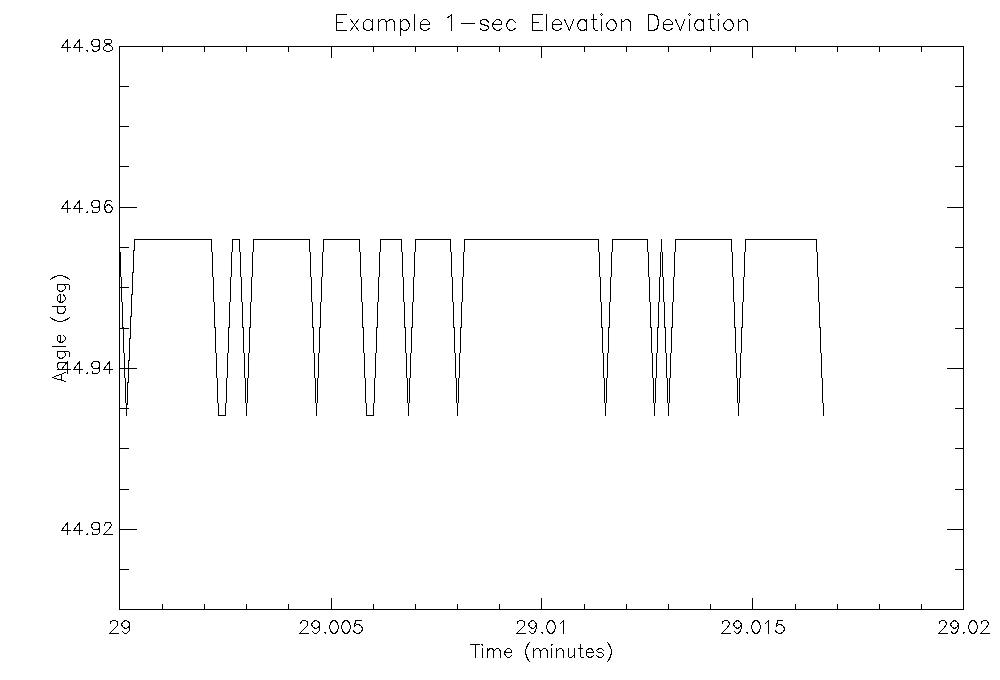
\includegraphics[width=1\linewidth]{appendix/img/campaign_results/earlyalt1sec.png}
		\caption{}
		\label{fig:sub:earlyalt1}
	\end{subfigure}
	\begin{subfigure}{0.45\textwidth}
		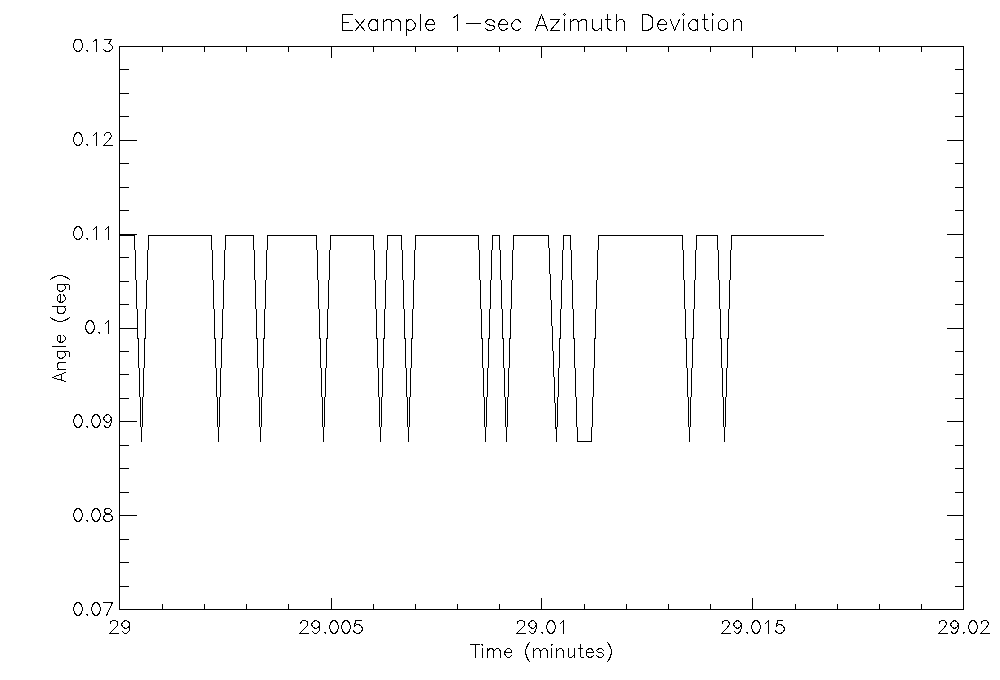
\includegraphics[width=1\linewidth]{appendix/img/campaign_results/earlyaz1sec.png}
		\caption{}
		\label{fig:sub:earlyaz1}
	\end{subfigure}
	\begin{subfigure}{0.45\textwidth}
		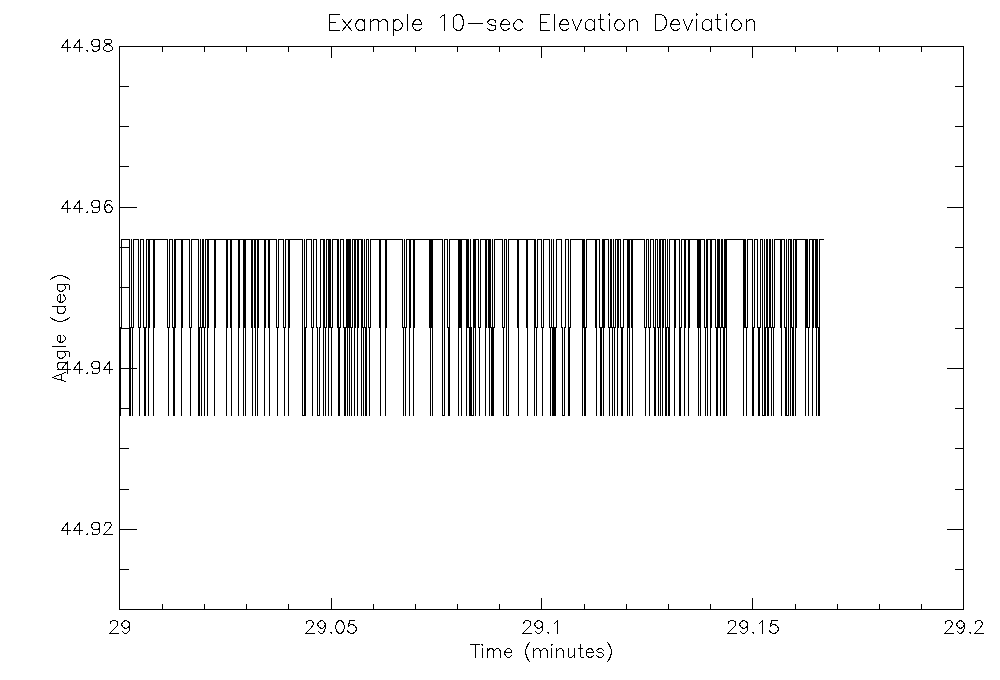
\includegraphics[width=1\linewidth]{appendix/img/campaign_results/earlyalt10.png}
		\caption{}
		\label{fig:sub:earlyalt10}
	\end{subfigure}
	\begin{subfigure}{0.45\textwidth}
		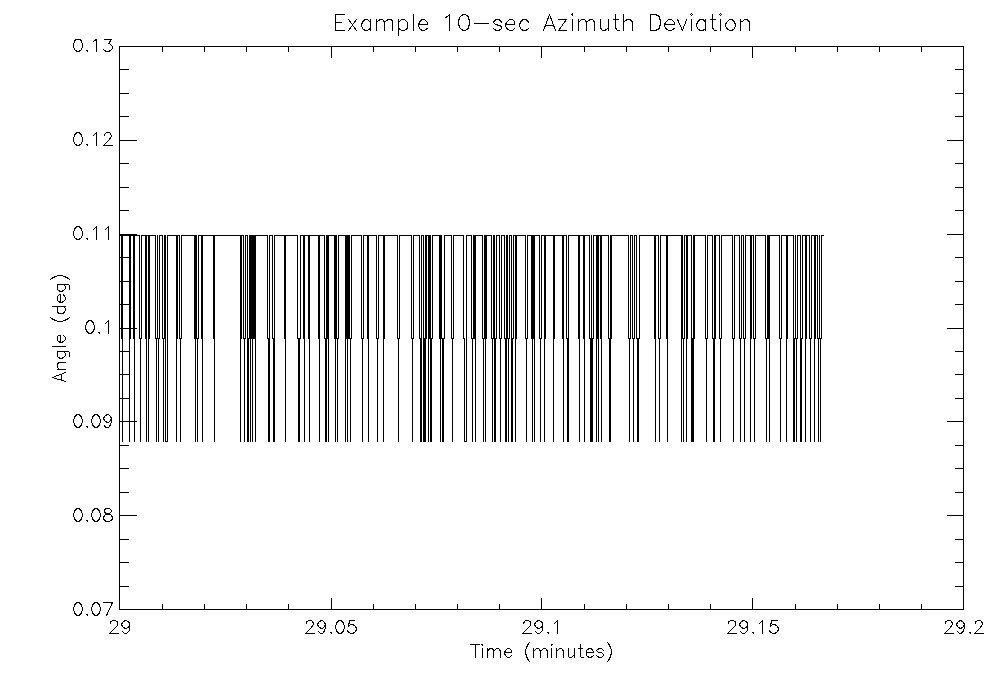
\includegraphics[width=1\linewidth]{appendix/img/campaign_results/earlyaz10sec.png}
		\caption{}
		\label{fig:sub:earlyaz10}
	\end{subfigure}
	\begin{subfigure}{0.45\textwidth}
		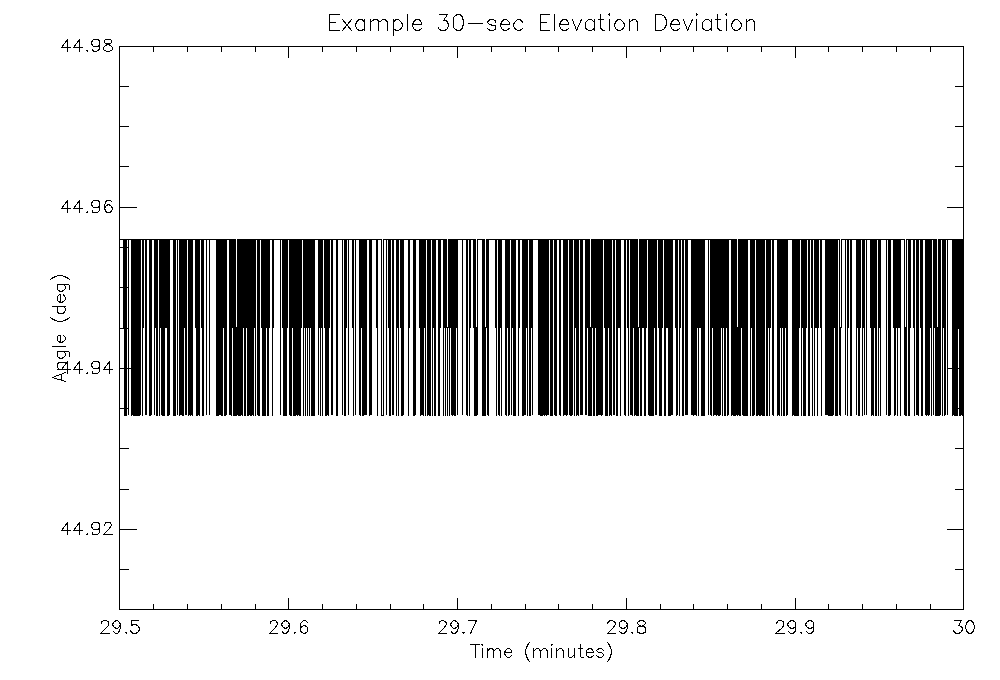
\includegraphics[width=1\linewidth]{appendix/img/campaign_results/earlyalt30.png}
		\caption{}
		\label{fig:sub:earlyalt30}
	\end{subfigure}
	\begin{subfigure}{0.45\textwidth}
		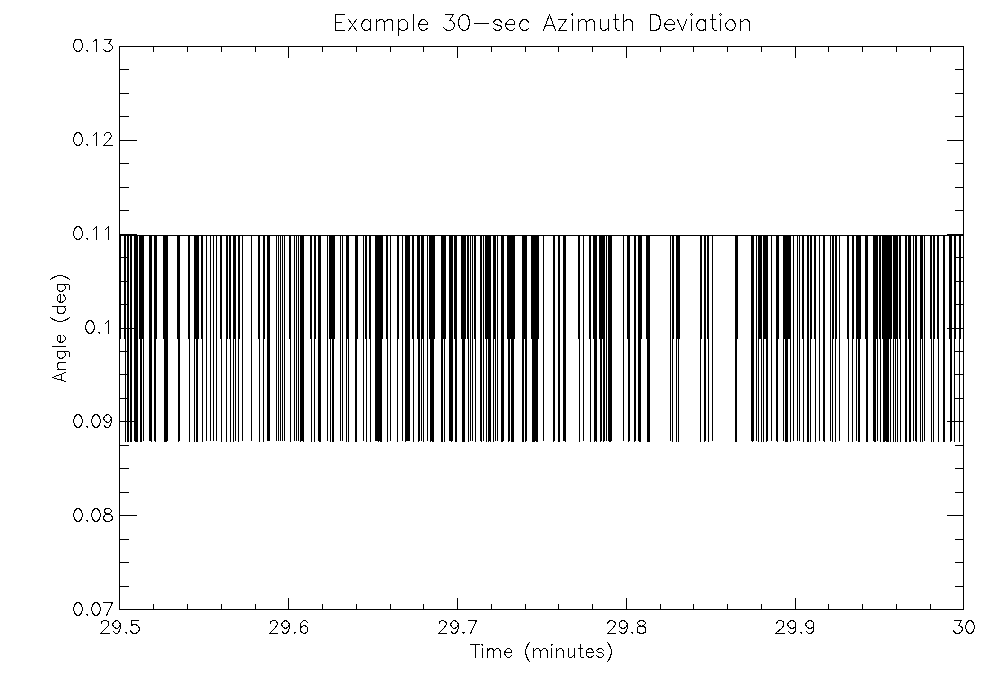
\includegraphics[width=1\linewidth]{appendix/img/campaign_results/earlyaz30sec.png}
		\caption{}
		\label{fig:sub:earlyaz30}
	\end{subfigure}
	\caption{Views of encoder data for successive time bins on both axes, early flight}
	\label{fig:earlyflight}
\end{figure}

\newpage
\begin{figure}[htbp]
\captionsetup[subfigure]{justification=centering}
\captionsetup{justification=centering}
    \centering
	\begin{subfigure}{0.45\textwidth}
		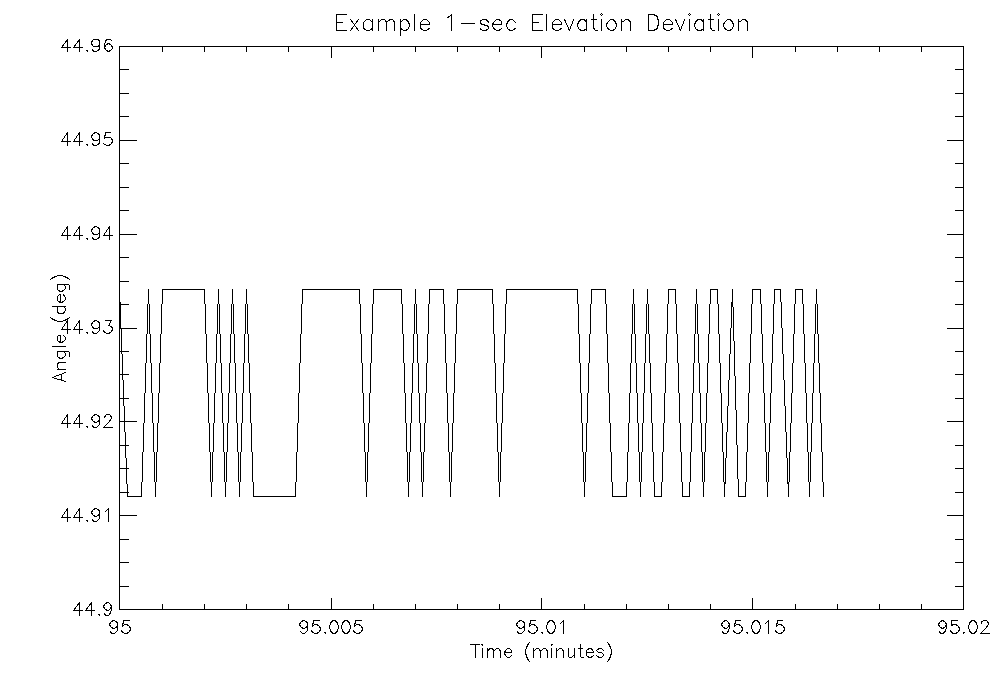
\includegraphics[width=1\linewidth]{appendix/img/campaign_results/latealt1sec.png}
		\caption{}
		\label{fig:sub:latealt1}
	\end{subfigure}
	\begin{subfigure}{0.45\textwidth}
		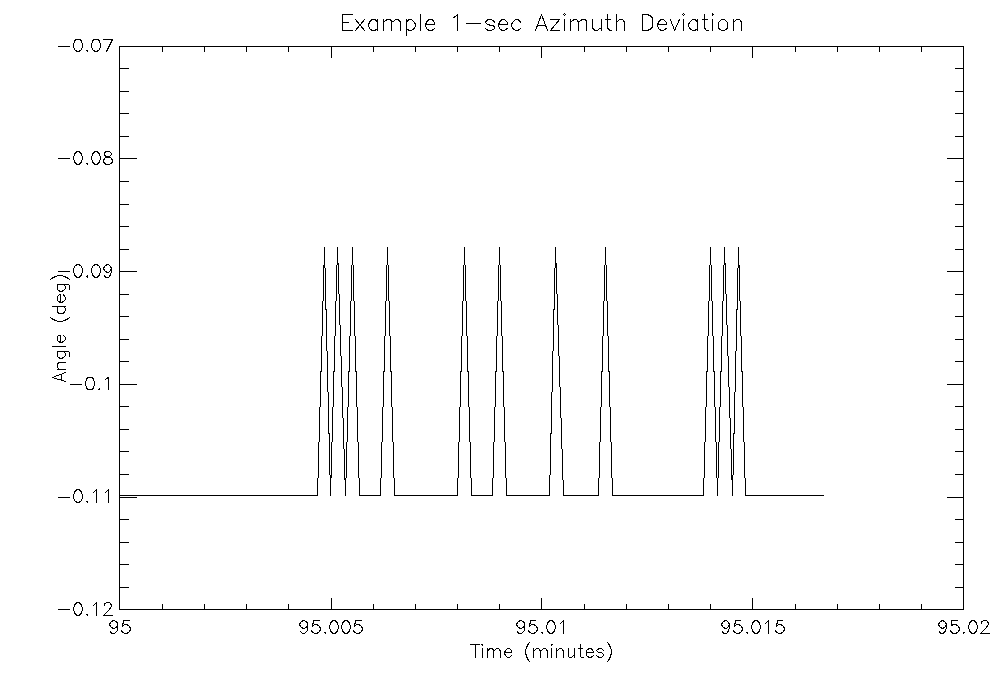
\includegraphics[width=1\linewidth]{appendix/img/campaign_results/lateaz1sec.png}
		\caption{}
		\label{fig:sub:lateaz1}
	\end{subfigure}
	\begin{subfigure}{0.45\textwidth}
		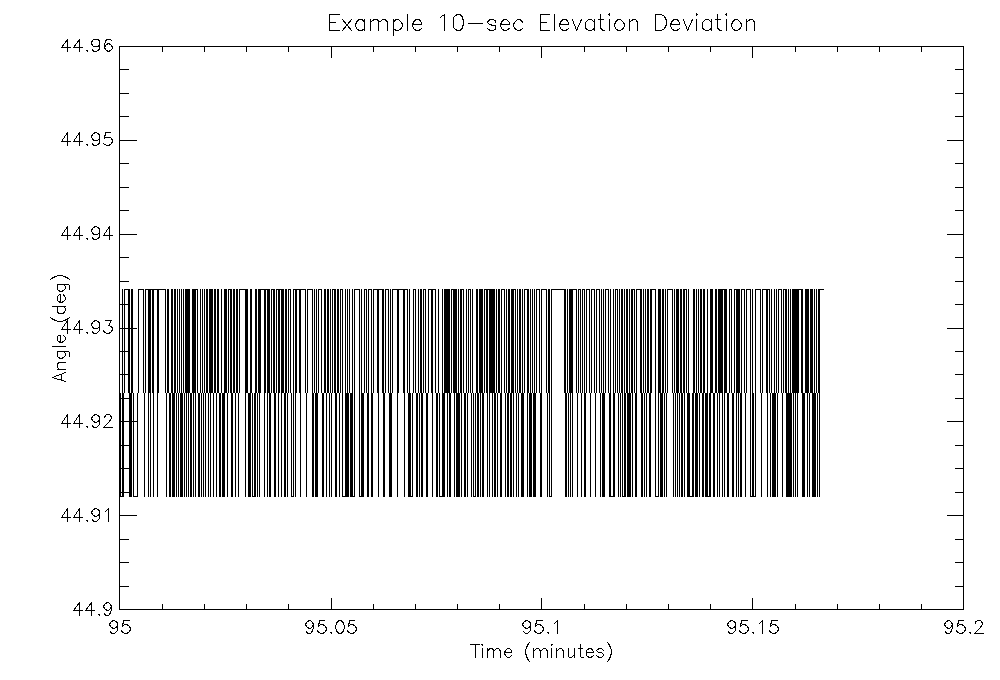
\includegraphics[width=1\linewidth]{appendix/img/campaign_results/latealt10sec.png}
		\caption{}
		\label{fig:sub:latealt10}
	\end{subfigure}
	\begin{subfigure}{0.45\textwidth}
		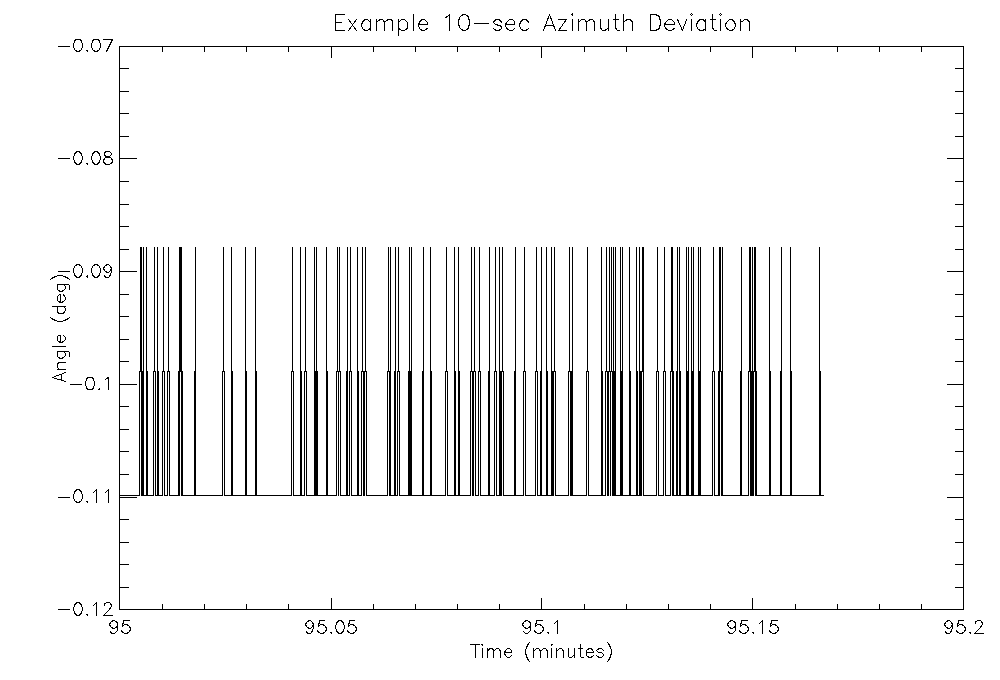
\includegraphics[width=1\linewidth]{appendix/img/campaign_results/lateaz10sec.png}
		\caption{}
		\label{fig:sub:lateaz10}
	\end{subfigure}
	\begin{subfigure}{0.45\textwidth}
		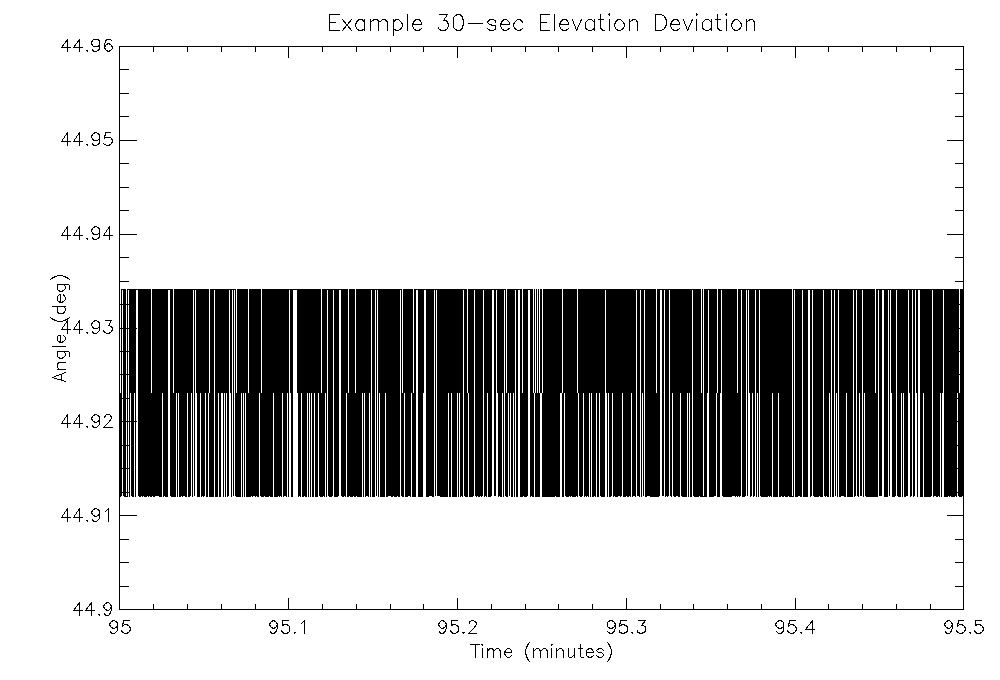
\includegraphics[width=1\linewidth]{appendix/img/campaign_results/latealt30sec.png}
		\caption{}
		\label{fig:sub:latealt30}
	\end{subfigure}
	\begin{subfigure}{0.45\textwidth}
		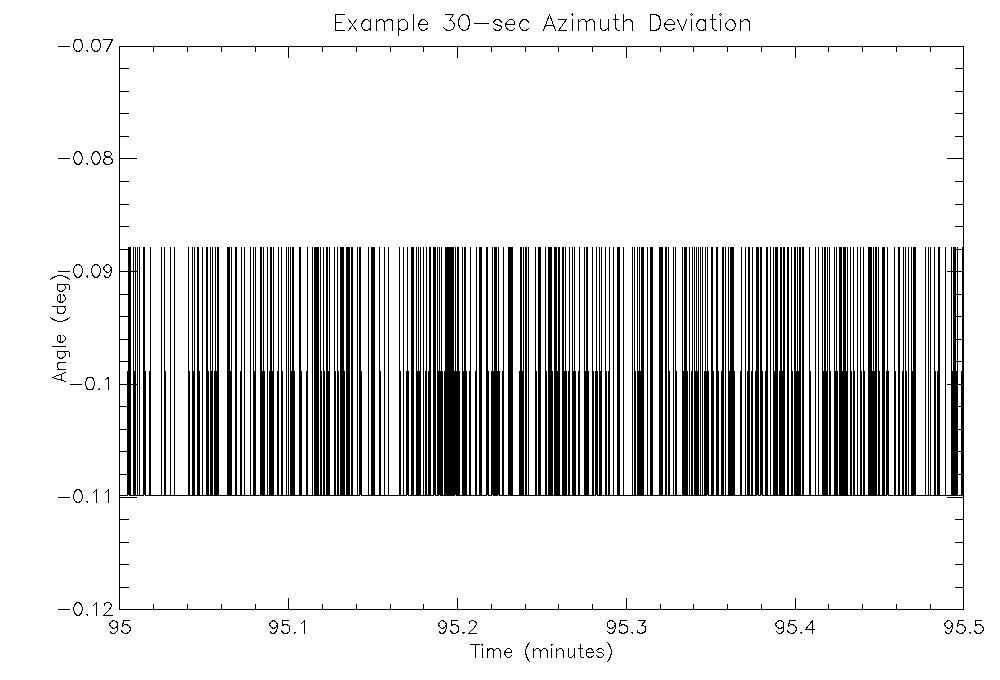
\includegraphics[width=1\linewidth]{appendix/img/campaign_results/lateaz30sec.png}
		\caption{}
		\label{fig:sub:lateaz30}
	\end{subfigure}
	\caption{Views of encoder data for successive time bins on both axes, late flight}
	\label{fig:lateflight}
\end{figure}

\newpage
\subsubsection*{Gyroscope and PID logs}

Figure \ref{fig:gyrodetail} shows gyroscope behaviour on shorter half-second and one-second timescales for each axis. 

\begin{figure}[htbp]
\captionsetup[subfigure]{justification=centering}
\captionsetup{justification=centering}
    \centering
	\begin{subfigure}{0.45\textwidth}
		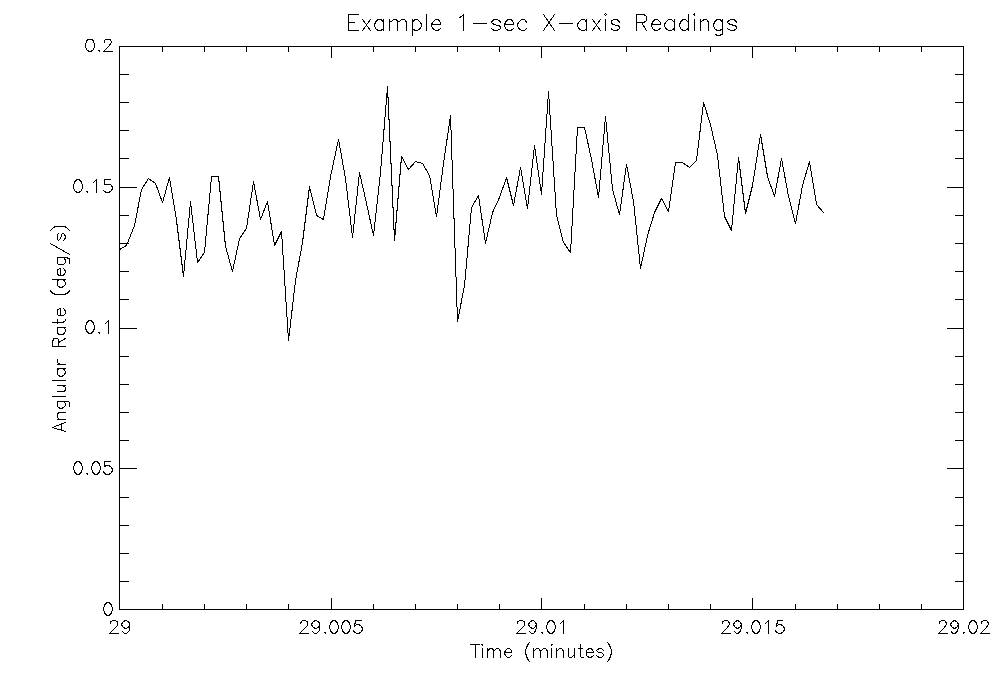
\includegraphics[width=1\linewidth]{appendix/img/campaign_results/gyrox1sec.png}
		\caption{}
		\label{fig:sub:gyrox1}
	\end{subfigure}
	\begin{subfigure}{0.45\textwidth}
		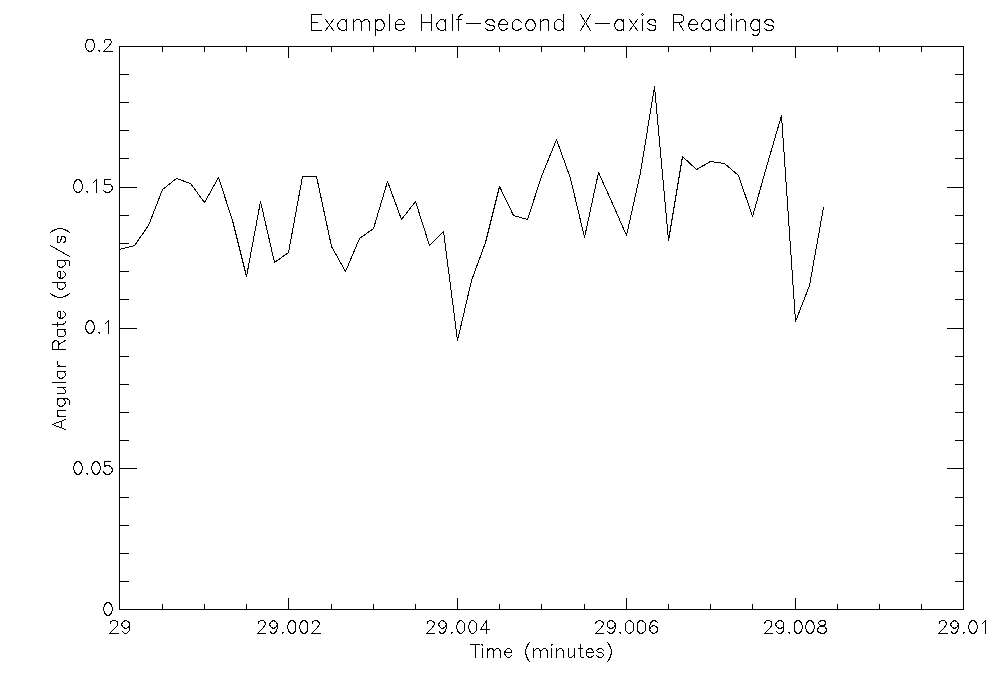
\includegraphics[width=1\linewidth]{appendix/img/campaign_results/gyroxhalfsec.png}
		\caption{}
		\label{fig:sub:gyroxh}
	\end{subfigure}
	\begin{subfigure}{0.45\textwidth}
		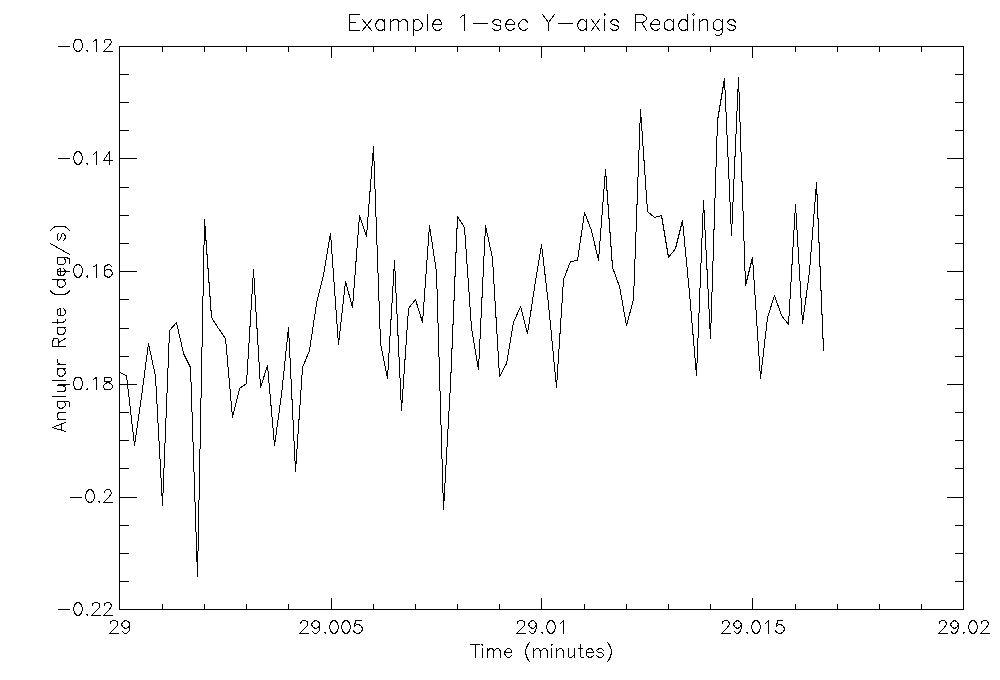
\includegraphics[width=1\linewidth]{appendix/img/campaign_results/gyroy1sec.png}
		\caption{}
		\label{fig:sub:gyroy1}
	\end{subfigure}
	\begin{subfigure}{0.45\textwidth}
		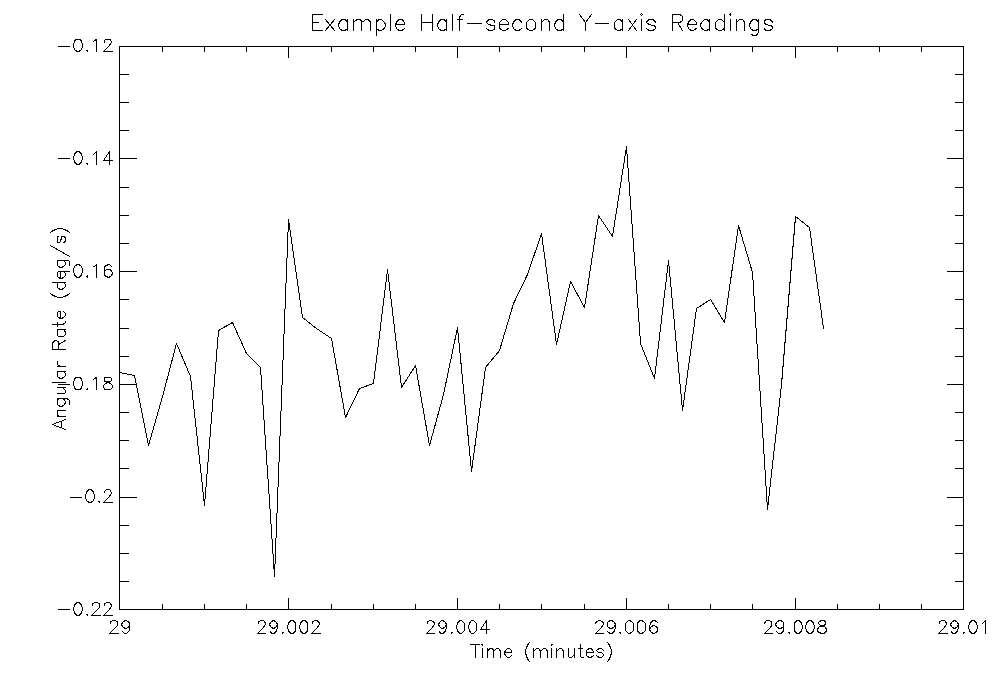
\includegraphics[width=1\linewidth]{appendix/img/campaign_results/gyroyhalfsec.png}
		\caption{}
		\label{fig:sub:gyroyh}
	\end{subfigure}
	\begin{subfigure}{0.45\textwidth}
		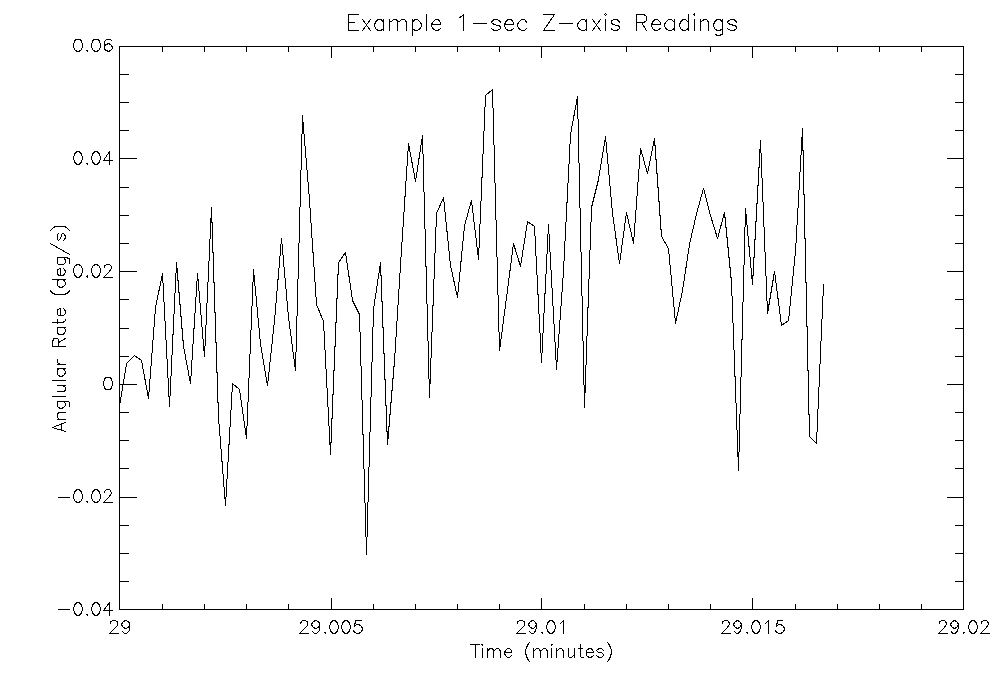
\includegraphics[width=1\linewidth]{appendix/img/campaign_results/gyroz1sec.png}
		\caption{}
		\label{fig:sub:gyroz1}
	\end{subfigure}
	\begin{subfigure}{0.45\textwidth}
		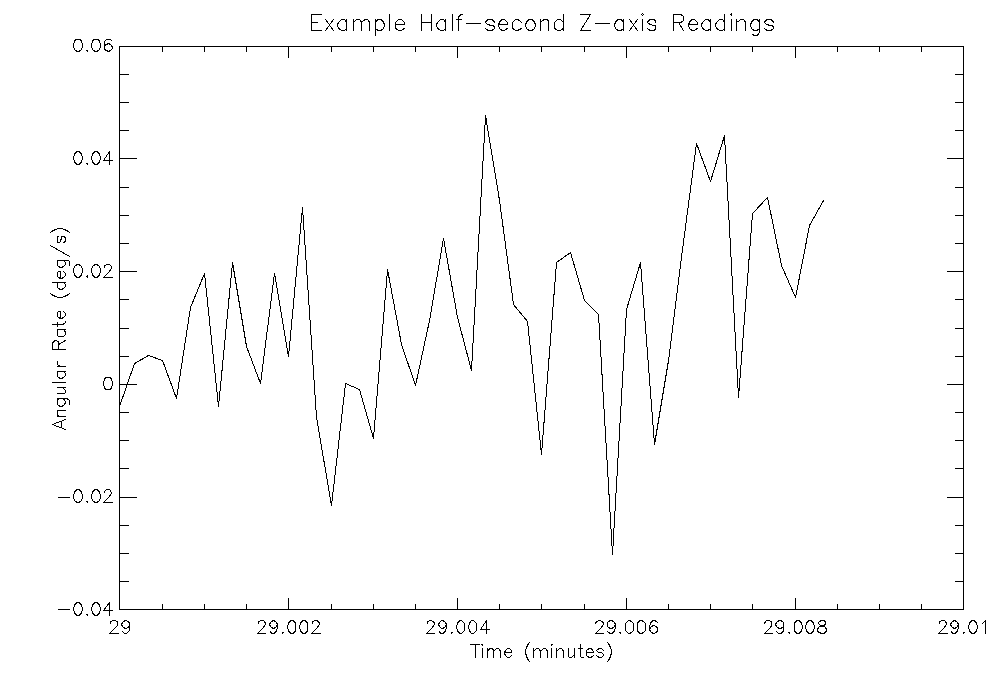
\includegraphics[width=1\linewidth]{appendix/img/campaign_results/gyrozhalfsec.png}
		\caption{}
		\label{fig:sub:gyrozh}
	\end{subfigure}
	\caption{Views of gyro data for each axis at one- and half-second bins}
	\label{fig:gyrodetail}
\end{figure}

Upon inspection it was noticed that the PID data recorded and presented in \ref{fig:PID} was the result of an error, wherein the azimuth data \ref{fig:sub:pidaz} was recorded twice. As such, only the PID azimuth data was considered to be compared against integrated gyroscope data.

\begin{figure}[htbp]
\captionsetup[subfigure]{justification=centering}
\captionsetup{justification=centering}
    \centering
		\begin{subfigure}{0.45\textwidth}
		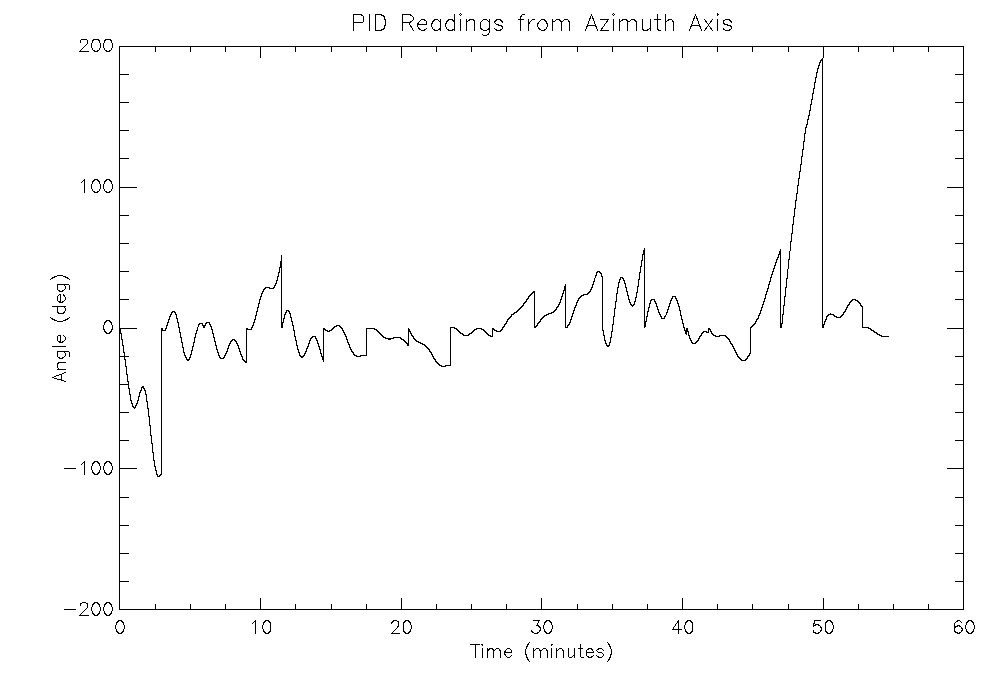
\includegraphics[width=1\linewidth]{appendix/img/campaign_results/pid_az.png}
		\caption{PID log recordings for the azimuth axis}
		\label{fig:sub:pidazvs}
	\end{subfigure}
	\begin{subfigure}{0.45\textwidth}
		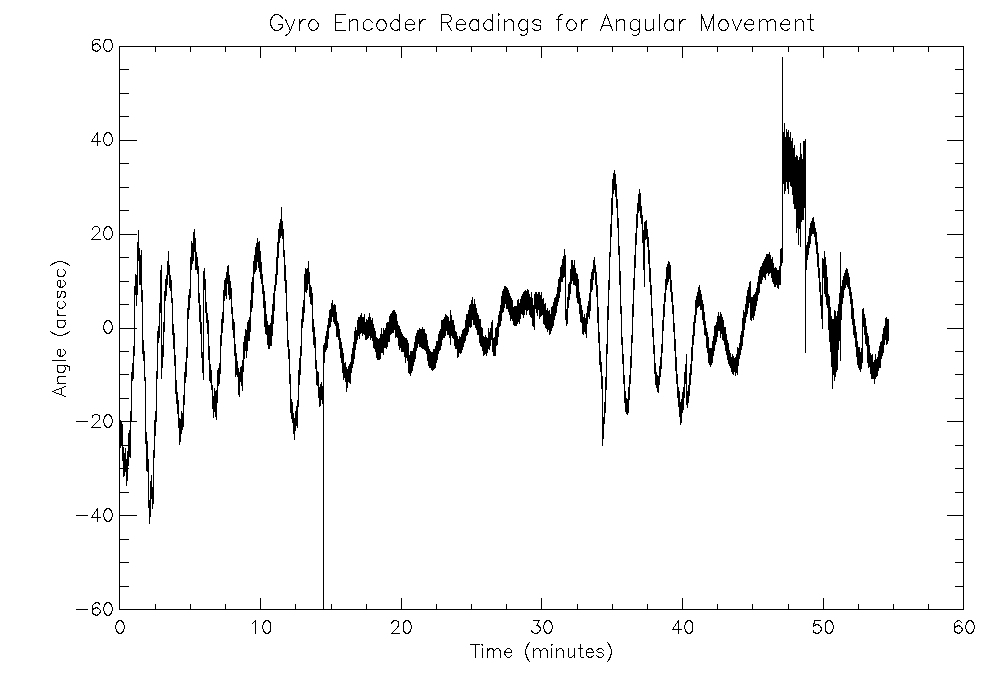
\includegraphics[width=1\linewidth]{appendix/img/campaign_results/gyroint.png}
		\caption{Integrated x-axis gyroscope data}
		\label{fig:sub:gyrointx}
	\end{subfigure}
	\begin{subfigure}{0.45\textwidth}
		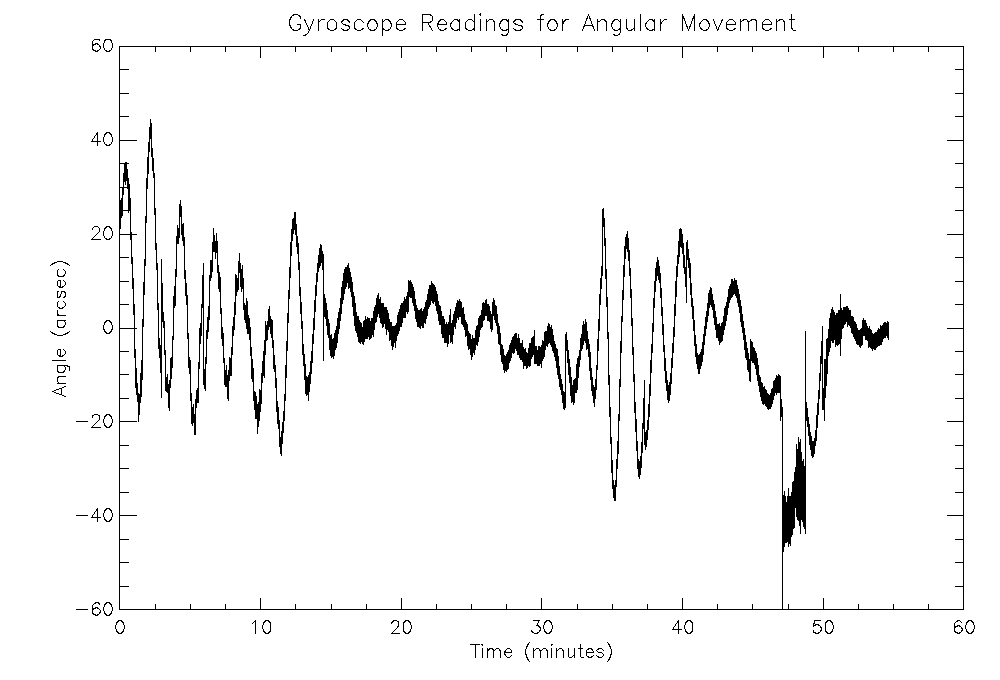
\includegraphics[width=1\linewidth]{appendix/img/campaign_results/gyrointy.png}
		\caption{Integrated y-axis gyroscope data}
		\label{fig:sub:gyrointy}
	\end{subfigure}
	\begin{subfigure}{0.45\textwidth}
		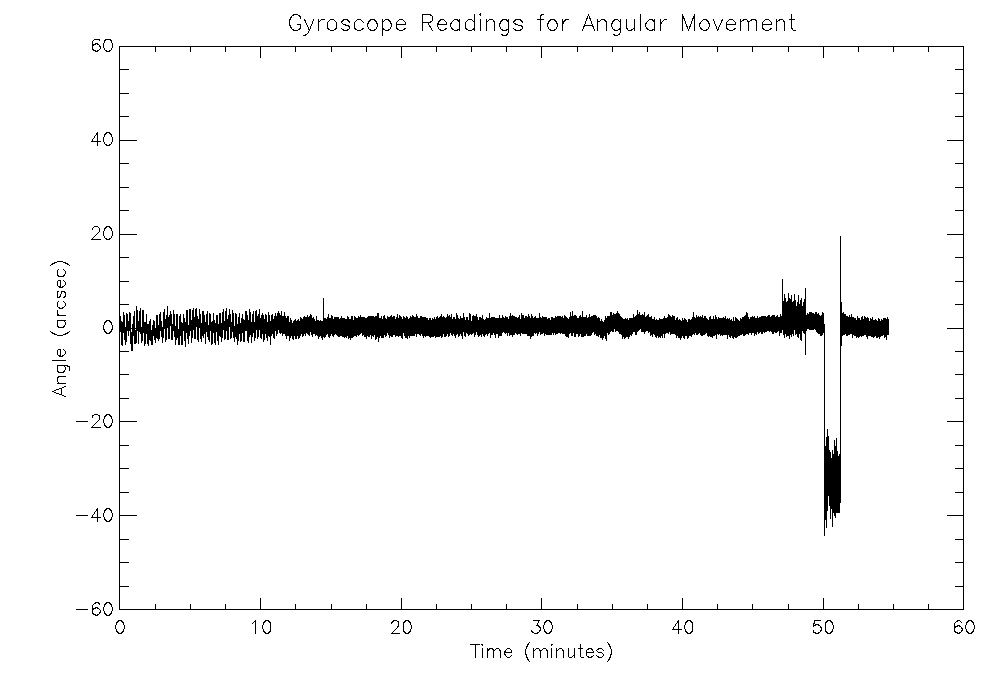
\includegraphics[width=1\linewidth]{appendix/img/campaign_results/gyrointz.png}
		\caption{Integrated z-axis gyroscope data}
		\label{fig:sub:gyrointz}
	\end{subfigure}
	\caption{Results from the PID log for the azimuth axis versus integrated gyroscope data for all axes.}
	\label{fig:PIDvsgro}
\end{figure}

